
\subsection{{Description}}

	{An 8-bit register utilizing D flip-flops serves as a digital storage unit, where each flip-flop corresponds to a single bit of data.} 
	
	{The register is structured with eight D flip-flops arranged in a cascading fashion, forming a sequential chain from the least significant bit (LSB) to the most significant bit (MSB).} 
	
	{The presence of the reset input allows for the complete clearing of the register, initializing all flip-flops to a predetermined state, commonly zero ("00000000" in this circuit design).} 
	
	{Synchronization is achieved through a clock signal, ensuring precise data capture at specified clock edges and mitigating signal propagation delays.} 
	
	{This 8-bit register plays a vital role in our digital logic circuit, as its output is an direct input to the arithmetic logic unit (ALU).}

\subsection{{Truth Table}}

	{An 8-bit register would ideally have 256 possible state values for some arbitary string of inputs "A" \& "B".}
	
	{Our choice of "A" \& "B" are the last 4 digits of my student number (50120\textbf{9136}) in hexadecimal converted to binary.}
	
	{$$\therefore A = (91)_{16} = (10010001)_{2}$$}
	
	{$$\therefore B = (36)_{16} = (00110110)_{2}$$}

	{The pair of inputs under consideration represent two among the 256 potential combinations achievable through an 8-bit D-flip-flop employed for input processing.}
	
	{In practice, when input A is applied, the D-flip-flop captures and retains the corresponding value until it is transmitted to the output during the subsequent rising edge. Notably, alterations to the output state exclusively occur on a rising edge, contingent upon the presence of a novel input.}
	
	{In the absence of a distinct input, the output remains unchanged unless a reset condition is invoked. This operational behavior underscores the discrete and controlled nature of input-output transformations within the described system.}

	\begin{table}[H]
		\centering
		\begin{tabular}{|c|c|c|c|}
		\hline
		\hline
			\textit{Reset} & \textit{Clock} & \textit{A} & $O(A, Clock, Reset)$ \\ 
		\hline
		\hline
			0 & 0 & 10010001 & 00000000 (If previous input exists, O = 10010001) \\ 
			\hline
			0 & 1 & 10010001 & 10010001 \\ 
			\hline
			1 & 0 & 10010001 & 00000000 \\ 
			\hline
			1 & 1 & 10010001 & 00000000 \\ 
		\hline
		\hline
    		\end{tabular}
    		\caption{Truth Table for the A input Register}
	\end{table}
	
	\begin{table}[H]
		\centering
		\begin{tabular}{|c|c|c|c|}
		\hline
		\hline
			\textit{Reset} & \textit{Clock} & \textit{B} & $O(B, Clock, Reset)$ \\ 
		\hline
		\hline
			0 & 0 & 00110110 & 00000000 (If previous input exists, O = 00110110) \\ 
			\hline
			0 & 1 & 00110110 & 00110110 \\ 
			\hline
			1 & 0 & 00110110 & 00000000 \\ 
			\hline
			1 & 1 & 00110110 & 00000000 \\ 
		\hline
		\hline
    		\end{tabular}
    		\caption{Truth Table for the B input Register}
	\end{table}

\subsection{{Block Diagram}}

	{To accommodate the requisite pair of 8-bit inputs, distinct registers are employed for the representation of values denoted as A and B. The application of the code prescribed in the laboratory guidelines yields illustrative block diagrams, as depicted in figure \ref{Latch}.}
	
	{Within this context, the inputs consist of "A," "Clock," and "Reset," collectively constituting the triad of input variables, while the resultant output ($O(B, Clock, Reset)$ from the \textbf{truth table}) is represented by "Q".}

	\begin{figure}[H]
		\centering
		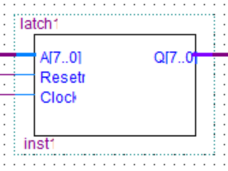
\includegraphics[width=10cm]{Pictures/Latch.png}
		\caption{{Block Diagram for the Registers}}
		\label{Latch}
	\end{figure}


\subsection{{Timing Diagram}}

	{}

	\begin{figure}[H]
		\centering
		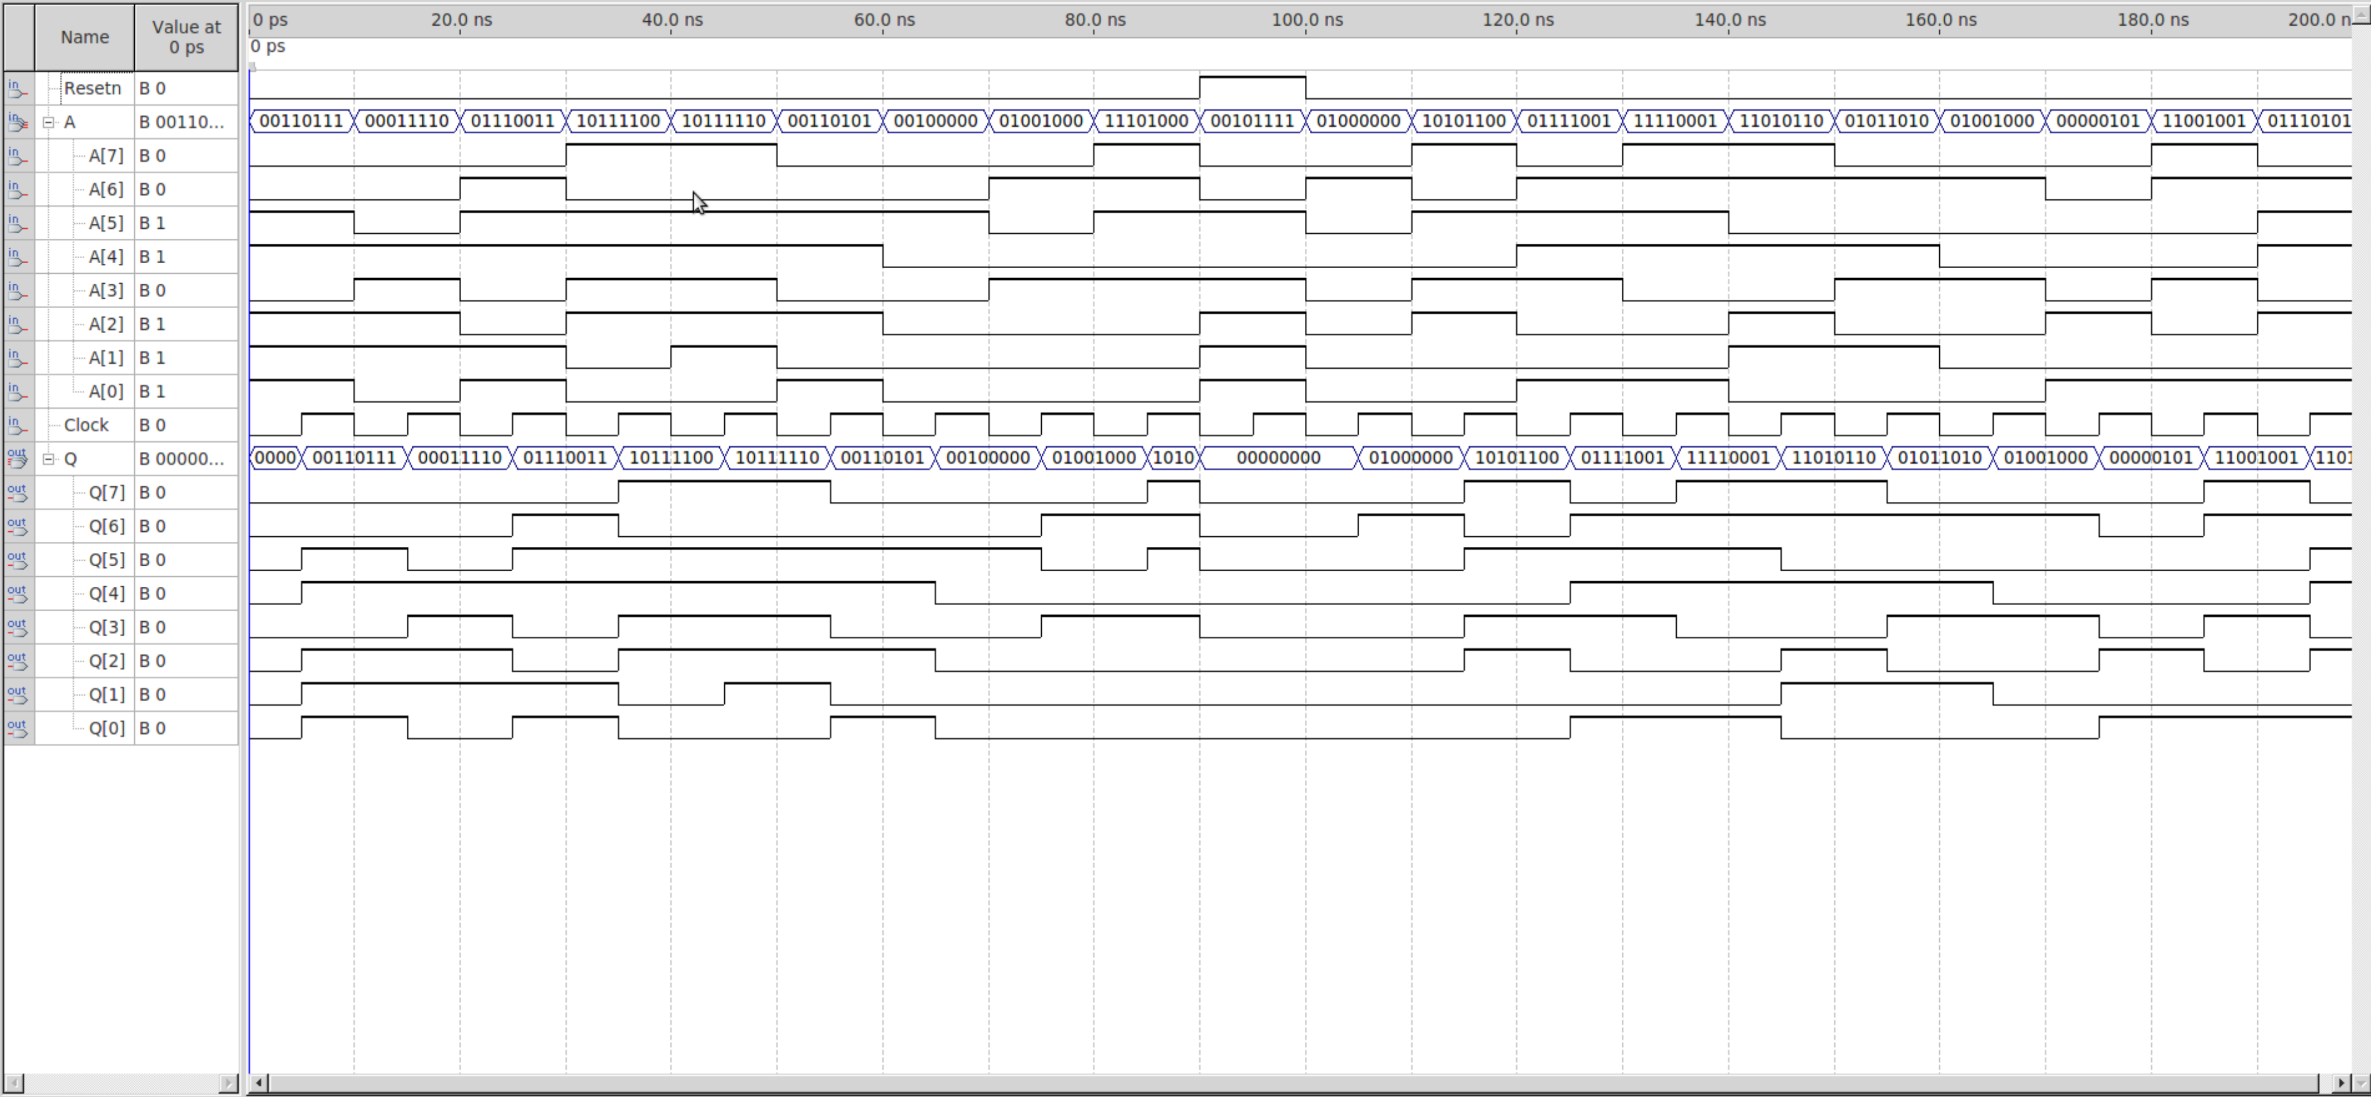
\includegraphics[width=15cm]{Pictures/RegisterWaveForm.png}
		\caption{{Timing Diagram for the Registers}}
		\label{Latch}
	\end{figure}
